%!TEX root = ../agi_mfwis415af4l.tex
\section{Benutzerhandbuch}
\label{concept}


\textbf{Installation der App} \\
Unter Android kann die App über ein an einen, mit Android Studio ausgestatteten, PC/Mac angeschlossenes Gerät (mind. API 15) installiert werden. Dazu muss das Projekt gestartet werden und bei dem Gerät das USB-Debugging aktiviert sein. Mit dem oben gelegenen „Play“ Button kann die App nun auf dem Gerät installiert werden.\\
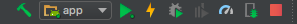
\includegraphics[scale=1]{img/androidstudio.jpg}\\
Die App wird nach der Installation automatisch auf dem Gerät gestartet.\\
\\
\textbf{Startseite} \\
Die Startseite ist übersichtlich aufgebaut und in drei große Bereiche eingeteilt. Im ersten Teil (von oben) befindet sich die Übersicht. Hier wird neben dem aktuellen Datum in der Mitte, link die eingenommenen Kalorien angezeigt. Diese werden aus dem aktuellen Tag zusammengerechnet angezeigt. Auf der rechten Seite befindet sich die für diesen Tag verbleibende Kalorienzahl, welcher ebenfalls berechnet wird. Zur optisch angenehmeren Darstellung und zur Erleichterung der Benutzung der App wird ebenfalls Fortschrittsbalken angezeigt welcher mit weiterer Kalorienzunahme voranschreitet. \\
Im zweiten und größten Feld spielt sich der Hauptteil der Aktivität ab, hier sind die vier verschiedenen Mahlzeiten zu sehen, „Frühstück“, „Mittagessen“, „Abendessen“ und „Snacks“. Mit den roten Plus Button lässt sich einfach ein Lebensmittel/Menü zur jeweiligen Mahlzeit hinzufügen. Es öffnet sich ein neues Fenster Hinzufügen. Das Datum ist hier ebenfalls wieder zu finden. In den folgenden beiden Spinnern kann man außerdem neu auswählen zu welcher Mahlzeit man das Lebensmittel/Menü hinzufügen möchte, um einen Fehler schneller zu korrigieren und das Lebensmittel/Menü welches in einem Auswahlmenü zur Verfügung steht. Anschließend muss nur noch die verzehrte Menge eingetragen werden. Die Anzahl an Kalorien wird unten automatisch angezeigt. Ist alles fertig eingetragen klickt man auf den Button „Hinzufügen“. Man gelangt nun automatisch zurück zu Startseite wo sich das Produkt nun in der passenden Ansicht der Mahlzeit befindet. Der Fortschrittsbalken, sowie beide Kalorienzahlen haben sich in der Kopfleiste ebenfalls angepasst.\\
Der letzte untere Teil besteht aus vier Buttons welche einfach zu erkennen und zu handhaben sind. Der erste Button öffnet die Kalenderansicht. Der zweite und dritte Button öffnet die Fenster Lebensmittel und Menü um diese jeweils hinzuzufügen, zu verändern oder zu entfernen. Mit dem letzten Button gelangt man zu der Profilansicht. \\
\\
\textbf{Kalenderansicht} \\
Der Kalender startet automatisch mit dem aktuellen Datum und ist in zwei Oberflächen eingeteilt. Oben befindet sich eine Kalenderansicht, durch welche durch einfache bekannte Tipp/Wischbewegungen navigiert werden kann. In der unteren Hälfte befindet sich die bereits aus der Startseite bekannte Mahlzeiten Ansicht. Diese ist dem App Design zugrunde gleich der Startseite aufgebaut. So findet man sich sofort in der gesamten App zurecht. \\
Mit der Auswahl eines Datums wird sofort die Mahlzeiten Ansicht angepasst und mit dem ausgewählten Datum angepasst. Man sieht nun die verzehrten Lebensmittel/Menüs von diesem Tag. Auf diese Möglichkeit lassen sich auch nachträglich Lebensmittel für einen bestimmten Tag eintragen, falls beispielsweise ein Nahrungsmittel vergessen wurde. Alternativ lassen sich auch eingetragene Lebensmittel entfernen oder anpassen, sowohl in der Menge als auch in der Position. Dadurch das sich die Ansicht Oberfläche dynamisch an die Menge der enthaltenen Lebensmittel anpasst ist ein angenehmes Scrollen in der App möglich. Der rote Button führt auch hier wieder zum Öffnen des Fensters Hinzufügen, welches bereits von der Startseite bekannt ist.\\
\\
\textbf{Lebensmittel} \\
Dieses Fenster ähnelt dem der Menüs und ist einfach und übersichtlich gestaltet. Die App kommt nach einer frischen Installation mit fünf Basis Lebensmitteln. Banane, Milch, Pizza, Reis und Schokolade. Diese sind in unterschiedlichen Mengen und Einheiten angegeben. Banane in Stück, Milch in Ml und Reis in Gramm beispielsweise. Die Ansicht der einzelnen Lebensmittel wächst mit der Anzahl an Lebensmitteln. Tippt man ein Lebensmittel an, öffnet man das Fenster Bearbeiten/Löschen hier kann man die Einträge des Lebensmittels verändern oder das Lebensmittel ganz löschen. Dies geschieht ganz einfach mit den jeweiligen Buttons „Löschen“ oder nach einer Änderung „Speichern“. Man kommt nun wie gewohnt automatisch zurück zum vorherigen Fenster. \\
Auf dem unteren Button „Lebensmittel hinzufügen“ lassen sich nun neue Lebensmittel hinzufügen. Die Felder die auszufüllen sind, sind Name des Lebensmittels, eine kurze Beschreibung, sowie eine Anzahl und die jeweilige Einheit pro Einnahme. Abschließend muss man nur noch die Kalorienanzahl für die jeweilige Menge des Lebensmittels eintragen und kann nun mit dem Button „Hinzufügen“ das Nahrungsmittel zu der Datenbank und zur späteren Auswahl hinzufügen. In der Lebensmittelliste befindet sich nun das neue Produkt. \\
\\
\textbf{Menü} \\
Wie schon gesagt besteht hier eine Ähnlichkeit zu den Lebensmitteln. Oben sind die bereits eingetragenen Menüs zu sehen und mit dem Button Hinzufügen kann man ein neues Menü hinzufügen. Drückt man auf den Button erscheint das Fenster Menü hinzufügen. Hier kann man zuerst einen Namen des Menüs eintragen, sowie eine kurze Beschreibung dazu addieren. In dem Feld Menübestandteile lässt sich mit dem bekannten roten Plus Button ein Lebensmittel zu diesem Menü hinzufügen. Hat man nun alle notwendigen Lebensmittel eingetragen kann man ganz simpel mit dem Button „Hinzufügen“ das Menü eintragen. Die Menüs stehen wie die Lebensmittel zum Eintragen in das Tagebuch im Dropdown Menü zur Verfügung. \\
Klickt man auf ein bestehendes Menü kann man dieses in dem folgenden Fenster problemlos bearbeiten. Nahrungsmittel können nun ergänzt, angepasst oder gelöscht werden um das Menü auf einen persönlichen Benutzer anzupassen.\\
\\
\textbf{Mein Profil} \\
Mit dem letzten Button der Startseite lässt sich das Benutzerprofil bearbeiten. Hier kann man seinen Namen eintragen und weitere benutzerspezifische Daten wie Größe und Gewicht. Für das Geburtsdatum ist ebenfalls ein Feld vorgesehen. Ein wichtiger Punkt ist das Kalorienlimit, welches in dem letzten Feld eigetragen werden kann. Die hier eingetragene tägliche Höchstzahl ist wichtig für die in der Startseite angewandten Zahlen und die Fortschrittsleiste, da diese sich hierauf berufen. Die Änderungen sind mit dem Button „Aktualisieren“ zu beenden, da dieser die eingetragenen Daten abspeichert und anpasst. \\
In diese Fenster lassen sich außerdem noch die Einheiten anpassen, mit dem Button „Einheiten Übersicht“. Klickt man auf den Button öffnet sich die Einheiten Übersicht, hier sieht man alle zur Verfügung stehenden Einheiten, kann diese anpassen und mit dem Button „Einheit Hinzufügen“ noch neue Einheiten in das Portfolio eintragen. Diese lassen sich selbstverständlich auch bearbeiten und löschen. \\
Mit einem weiteren Button „Statistische Auswertungen“ öffnet sich das Fenster der statistischen Auswertungen. Hier wird eine Übersicht über die durchschnittlich zu sich genommenen Kalorien der letzten 7, 14 oder 30 Tage gegeben.
